\section{Study of the Italian territory}

This section is a demographic analysis of Italian situation. We want to analyse how population is distributed throughout the country to later show how this aspect affects accessibility to healthcare services.

Figure \ref{fig:pop_by_region} shows how population is distributed on a regional level, classifying each region with a graduated scale based on the total inhabitants of the region.
Five classes have been defined, assigning each class the same interval.
\footnote{The Sturges's rule was followed, which suggest the number of bins to define when categorizing data.
	It states
	\begin{equation*}
		k = log_2 n +1
	\end{equation*}
	where $k$ represents the number of bins to be defined and $n$ the total number of elements.}
	
We can see from the figure that Lombardia is largely the most populated region, while Valle d'Aosta, Molise and Basilicata are the least populated.


\begin{figure}[tbp]
	\centering
	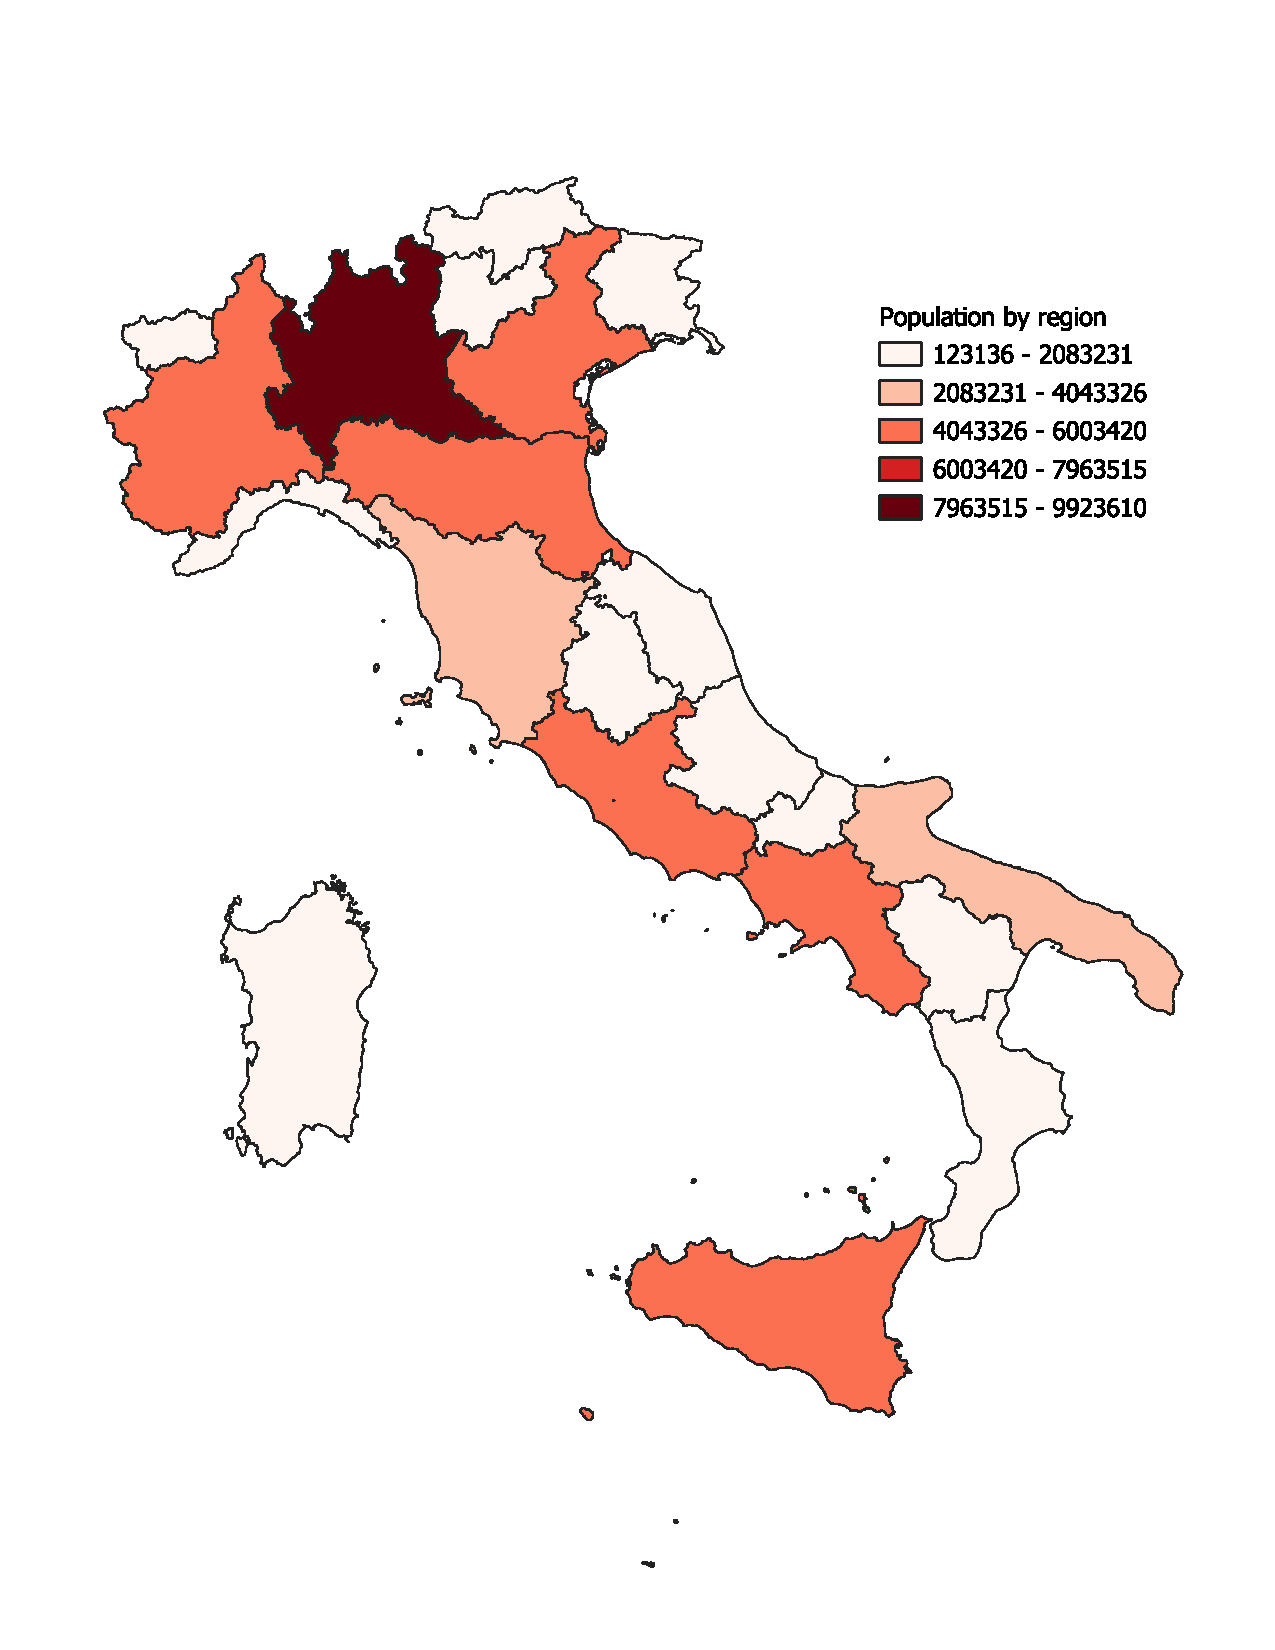
\includegraphics[width=0.8\textwidth]{img/regioni per popolazione.pdf}
	\caption{Italian population by region}
	\label{fig:pop_by_region}
\end{figure}

\begin{figure}[tbp]
	\centering
	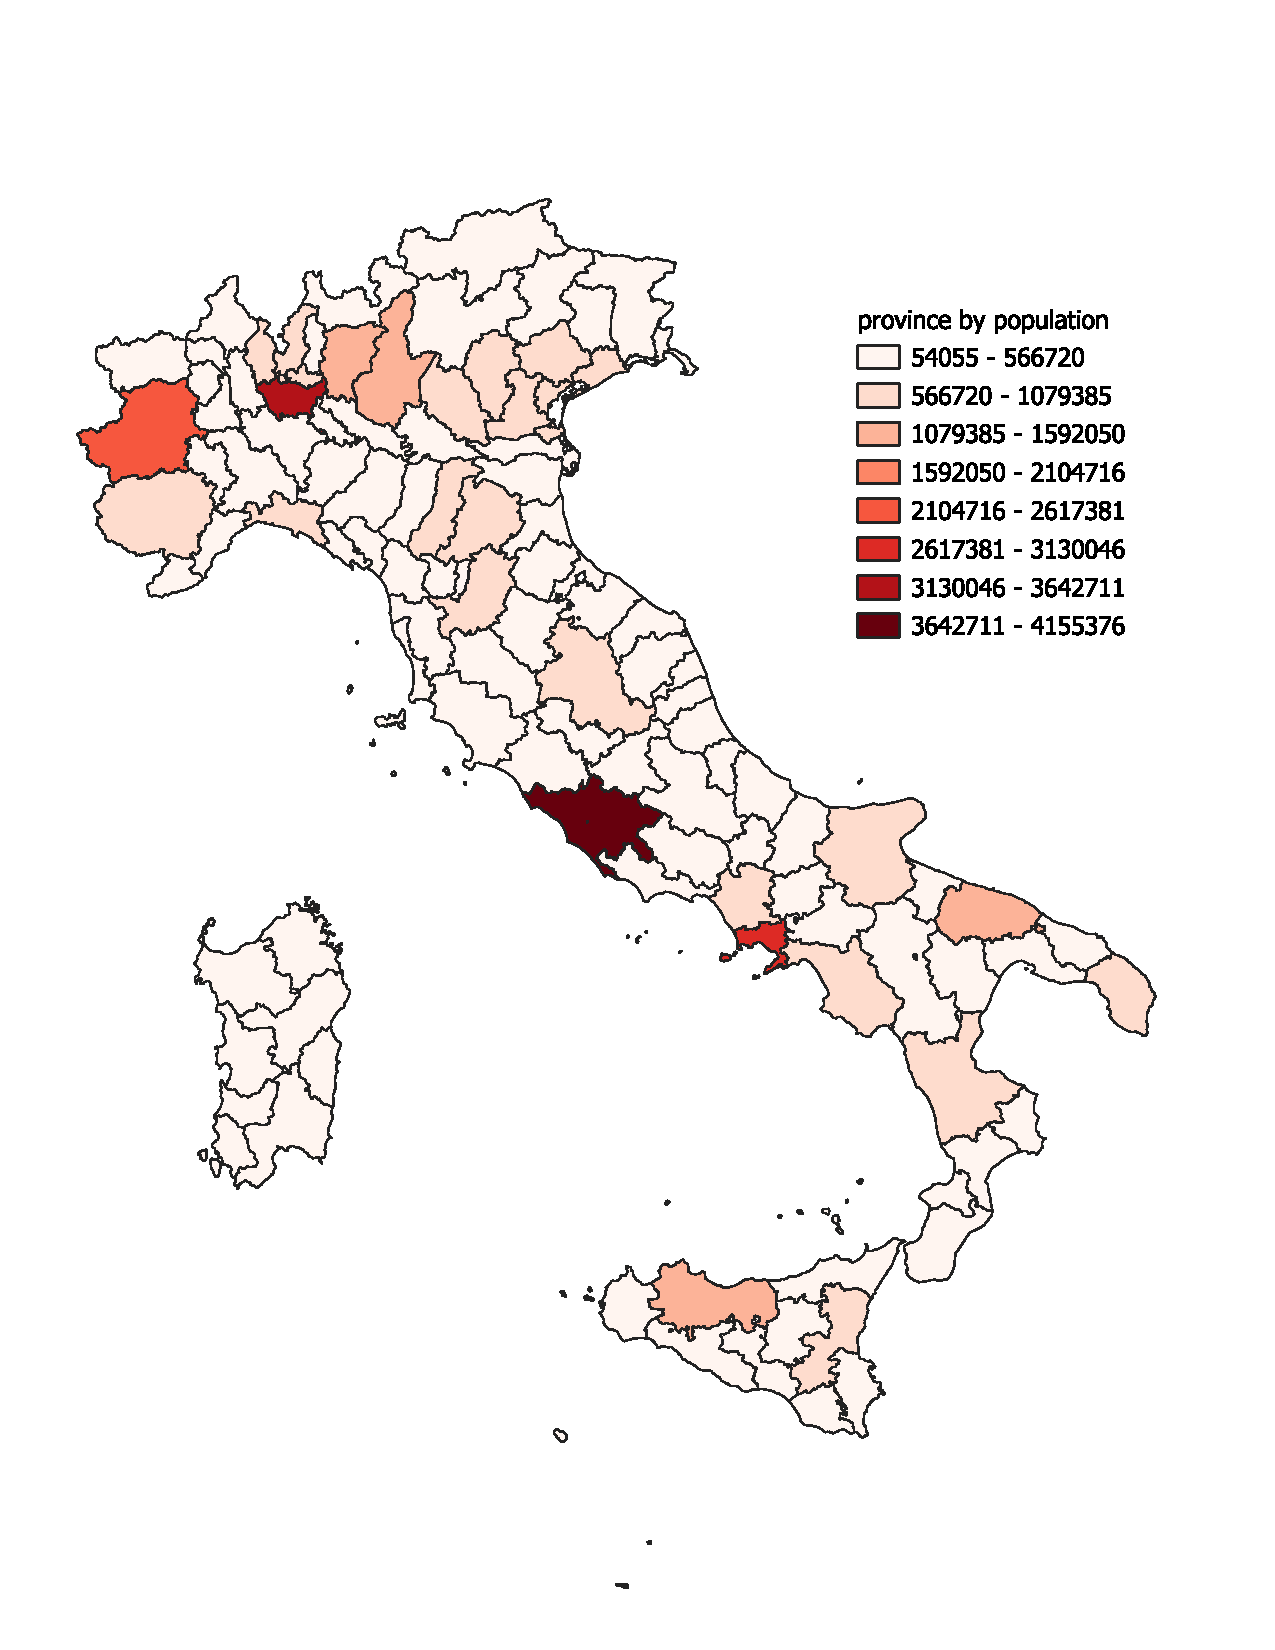
\includegraphics[width=0.8\textwidth]{img/province per popolazione.pdf}
	\caption{Italian provinces by population}
	\label{fig:pop_by_prov}
\end{figure}

By increasing the resolution we can analyse how the population is distributed at the municipal level.
The graph on Figure \ref{fig:pop_by_comm} is very right-skewed, meaning that the great majority of Italian population lives in little municipalities, smaller than 50 thousand inhabitants.
The graph is so right-skewed we can not even see other columns.



\begin{figure}[tbp]
	\centering
	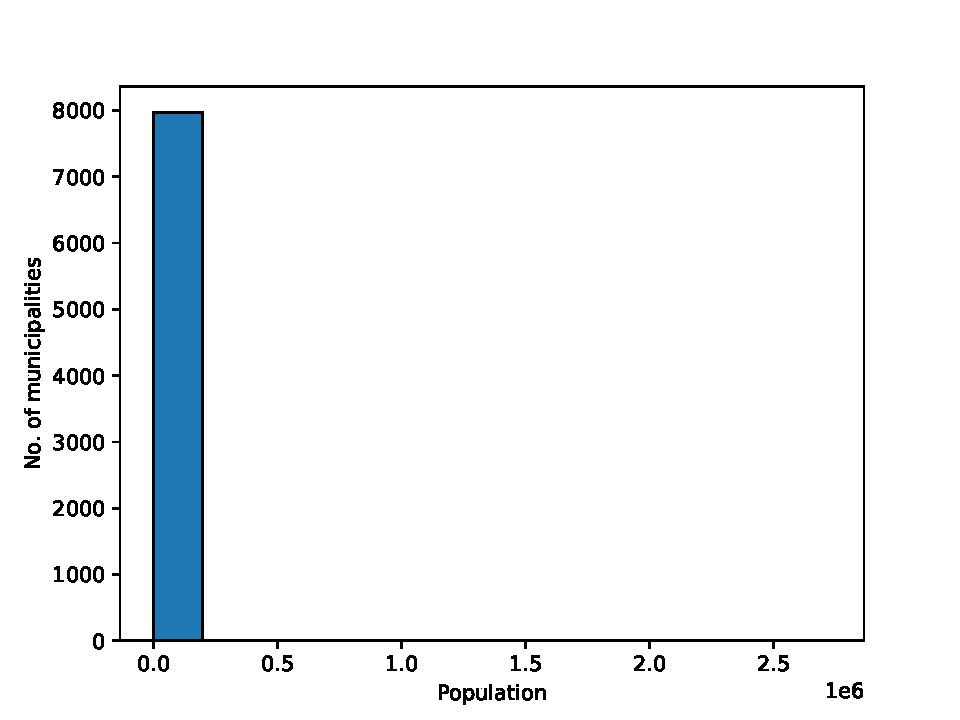
\includegraphics[width=0.8\textwidth]{img/pop_by_comm_hist.pdf}
	\caption{Distribution of population by municipality}
	\label{fig:pop_by_comm}
\end{figure}

\begin{figure}[tbp]
	\centering
	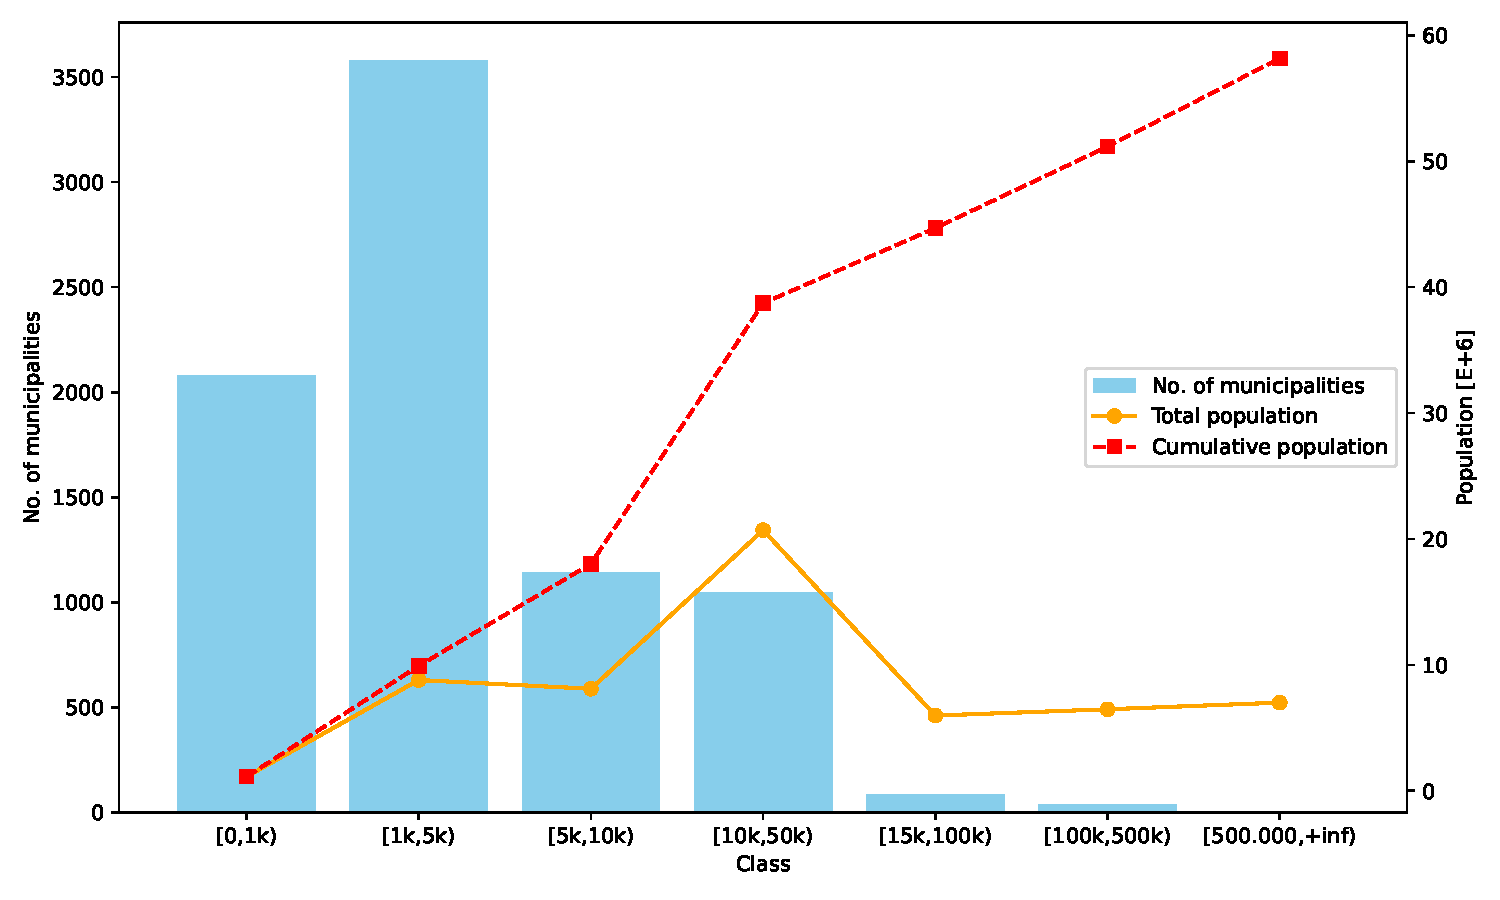
\includegraphics[width=\textwidth]{img/numOfComm_by_class_v2.pdf}
	\caption{Distribution of Italian communes by population and total population living in communes of that class}
	\label{fig:comm_by_class}
\end{figure}


\begin{table}[tbp]
	\centering
\begin{tabular}{rccc}
	\toprule
	Class & No. communes & Total pop. & \% on total\\
	\midrule
	< 1.000 & 2081 & 1120526 & 1.93\\
	1.000 – 4.999 & 3580 & 8795876 & 15.12\\
	5.000 – 9.999 & 1142 & 8101451 & 13.93\\
	10.000 – 49.999 & 1048 & 20700471 & 35.59\\
	50.000 – 99.999 & 88 & 5973913 & 10.27\\
	100.000 – 499.999 & 38 & 6472224 & 11.13\\
	>= 500.000 & 6 & 7001822 & 12.04\\
	\bottomrule
\end{tabular}
	\caption{Distribution of Italian communes by population.\\
		For each category:
		number of municipalities falling within that class,
		total population residing in those municipalities,
		percentage of the national population contained in each class}
	\label{tab:comm_by_class}
\end{table}

% TODO possibile inserire un Treemap